% Please do not change the document class
\documentclass{scrartcl}

% Please do not change these packages
\usepackage[hidelinks]{hyperref}
\usepackage[none]{hyphenat}
\usepackage{setspace}
\doublespace

% You may add additional packages here
\usepackage{amsmath}
\usepackage{graphicx}
\usepackage{wrapfig}
\graphicspath{ {images/} }


% Please include a clear, concise, and descriptive title
\title{A Comparison of Procedural Content Generators and Which Provides More Variety and Extensibility for an Indie Development Team} 

% Please do not change the subtitle
\subtitle{COMP110 - Computer Architecture Essay}

% Please put your student number in the author field
\author{1507516}

\begin{document}

\maketitle


\abstract{This paper will evaluate and compare three articles; A Rhythm-Based Level Generator for 2-D platformers \cite{smith2009}, Procedural Content Generation Using Occupancy-Regulated Extension \cite{mawhorter2010} and Procedural Content Generation Using Patterns as Objectives \cite{dahlskog2014}. These articles all have their own techniques to procedurally generate content for a 2-D platformer. This article recommends that Launchpad: A Rhythm-Based Level Generator is the most appropriate Procedural Content Generator (PCG) for an indie developer that would like to implement a 2-D platformer, based on variety and extensibility. These are important metrics because variety allows for more re-playability and extensibility allows the game to grow without a lot of performance issues.}


\section{Introduction}

The way in which we use Procedural Content Generators (PCG) to develop content for games is a vital part of the video game design process. With the recent release of popular procedurally generated 2-D games, such as \textit{Terraria}, \textit{Starbound} and \textit{Spelunky}, it is important to choose a procedural content generator that suits your needs. For the context of this paper, the indie developers would like to implement a PCG that can be integrated into the game engine, and compile the level at runtime on the PC platform.

The work is motivated by the complexity and variety of all the different approaches to Procedural Content Generation, and this paper aims to provide a comparison of three different papers and make a recommendation based on the extensibility and variety of each PCG. 

The reason why these three PCG articles were chosen was because they are all designed to generate levels in the style of Super Mario Bros (SMB).
The three articles are:

Launchpad: A Rhythm-Based Level Generator for 2-D platformers \cite{smith2009} \par

Procedural Level Generation Using Occupancy-Regulated Extension \cite{mawhorter2010} \par

Procedural Content Generation Using Patterns as Objectives \cite{dahlskog2014} \par

Variety is being measured by \textit{Linearity} and \textit{leniency} \footnote{leniency is how forgiving the level is to the player, e.g. levels with less obstacles or enemy's are more lenient. Linearity is a measure of the varying geometry of a level} which are metrics proposed by Smith and Whitehead \cite{smith2010}. Extensibility is being measured by how much control the developer has over the PCG and how the addition of content added to the game will affect the performance of the PCG.


\section{Review of Procedural Content Generation Articles}

\subsection{Launchpad: A Rhythm-Based Level Generator}

Launchpad generates levels out of small segments called ``\textit{rhythm groups}''  which are short, non-overlapping areas that contain a challenge for the player. I.e. a series of quick jumps or jumping back and forth between platforms. The rhythm groups are generated using a 2 tiered grammar \footnote{Grammar in this context meaning a set of rules for rewriting strings, which forms the basics of how procedural content generation works \cite{shaker2015}.} based approach.

The first stage of this creates a set of beats that correspond to a player action. This works well because it means the game can be improved by the addition of varying player actions. Furthermore each beat can be very different from the last beat, allowing for a lot of variety.
The second stage takes the player action and creates geometry based on its parameters, this is then added to the level as a ``rhythm group''. 

To achieve guaranteed playability of levels, Launchpad takes into account a set of parameters that determine how the player moves, e.g. the maximum speed the player can move, how high they can jump etc \cite{smith2012web}. This means that each level that is generated does not create sections which the player cannot pass. Furthermore designers are able to have a lot more control over the design of player movement without having to be concerned with level geometry, thus increasing the extensibility of the PCG.


\subsection{Procedural Level Generation Using Occupancy-Regulated Extension}

Occupancy-Regulated Extension (ORE) is able to generate levels without knowing anything about how the game works. This method works by using a library of chunks and assembling them based on a complex set of parameters. 

This algorithm generates the content in 3 stages, firstly it selects the location at which to start generating geometry. It then selects chunks from the library that is then tested with its filtering and selection algorithms to see if it is appropriate to place at that location. Lastly, that chunk is integrated within the existing content.

Compared to Launchpad, this method requires a large amount of human authored content to be available in order to get a varied level. Furthermore, this method is not very extensible as the more items are added to the library the longer it takes to generate a level. Even after the level is generated, it still requires a large amount of post-processing to make the game playable.\cite{mawhorter2010}

However when done correctly with the right settings, this approach can generate some very creative and complex levels as seen in figure \ref{fig:PCG} and \ref{fig:ocupancyfig2} . This is especially useful when creating exploration games.

\begin{figure}[t]
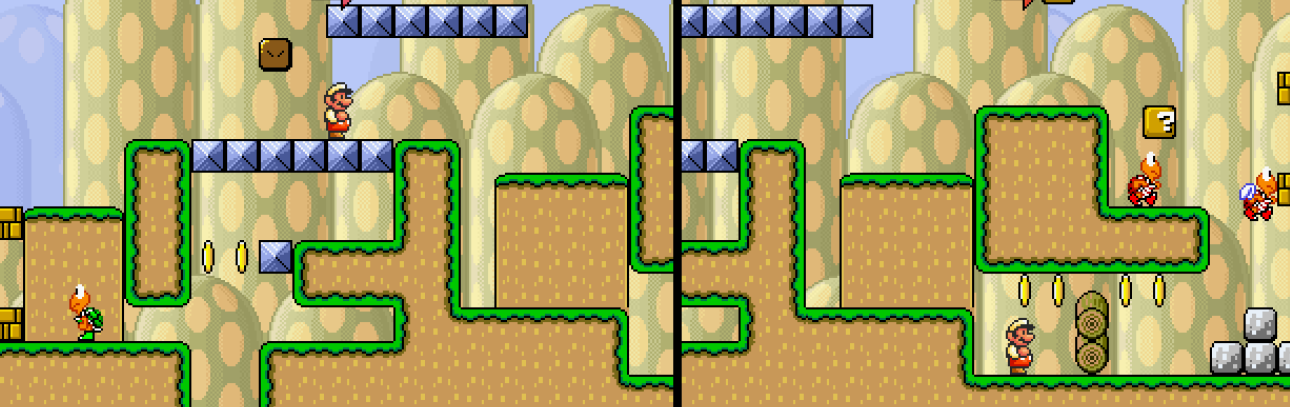
\includegraphics[width=8cm]{occupancy-complex}
\centering
    \caption{This shows some of the complex levels that the occupancy-regulated extension method can create. (image from \cite{mawhorter2010})}
    \label{fig:ocupancyfig2}
\end{figure}


However this approach does not guarantee playable levels, which for this context is not a desirable property.

\subsection{Procedural Content Generation Using Patterns as Objectives}

Dahlskog and Togelius \cite{dahlskog2014} take an interesting approach for this PCG. By looking for patterns in the way levels are structured in an original game such as SMB, and then analyzing that level design to generate levels that use the same level design techniques. This means that the levels can maintain a high quality, but still contain variation.

\begin{figure}[h]
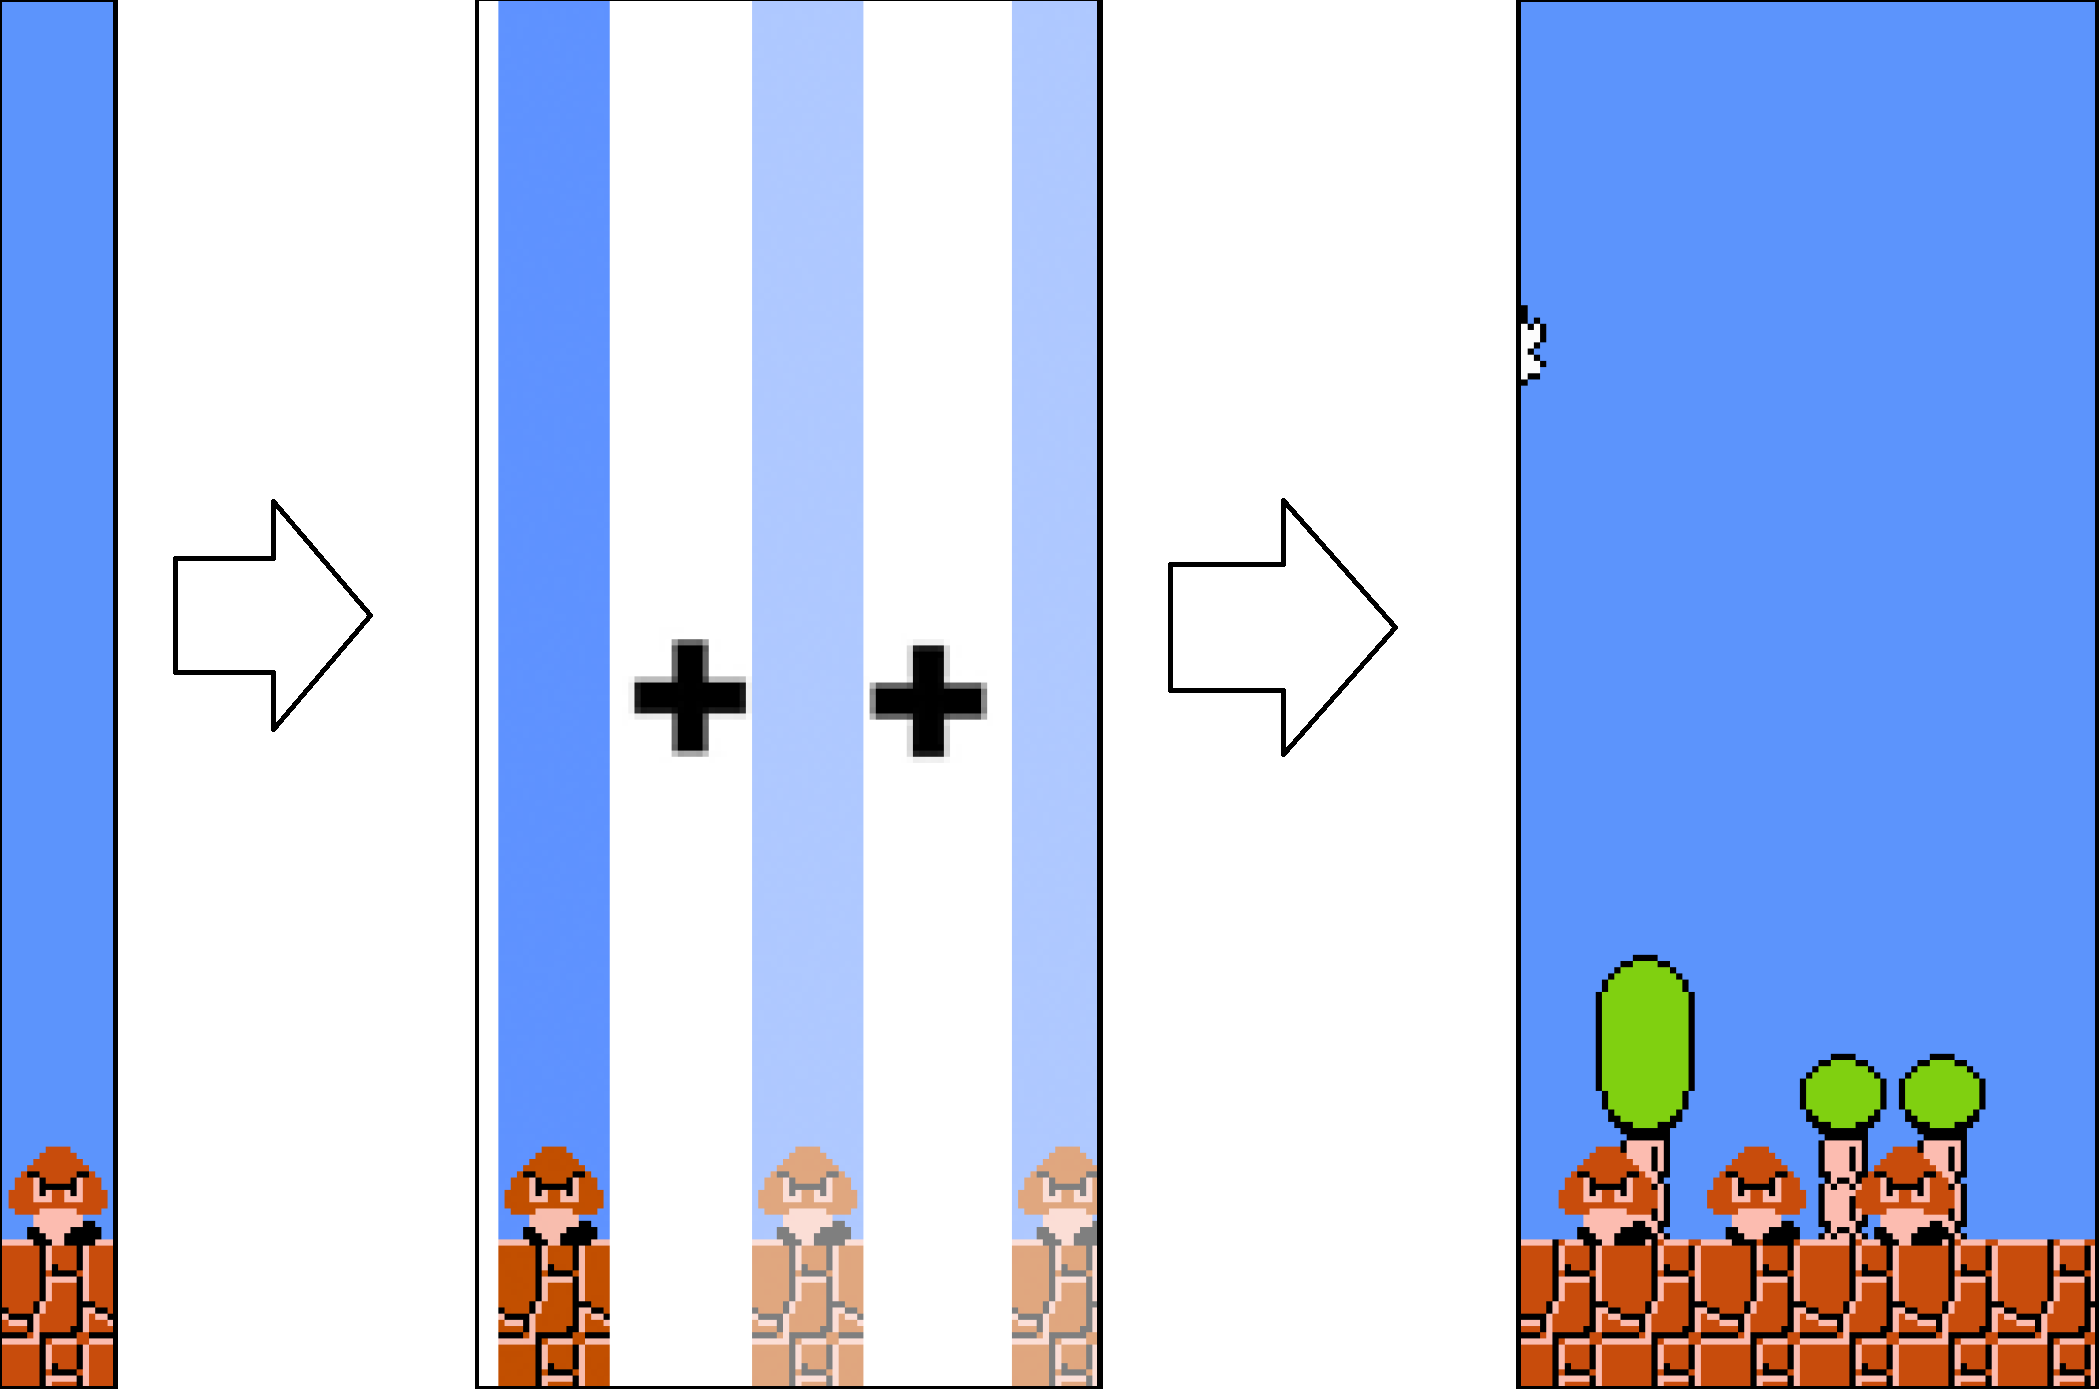
\includegraphics[width=8cm]{ocupancy1}
\centering
    \caption{The far left image is a micro-pattern containing a goomba which is then combined to form a meso-pattern in the far right image. (Figure from \cite{dahlskog2014})}
    \label{fig:ocupancyfig}
\end{figure}

This method works by identifying ``micro-patterns'' and ``meso-patterns'' in an existing game, such as SMB. Micro-patterns are a vertical 1-block wide slice of the level as shown in figure \ref{fig:ocupancyfig}, and meso-patterns are the way in which micro-patterns are arranged. The generator then uses the micro-patterns as building blocks to generate a new level.


\section{Comparison and Recommendation}

\begin{figure}[h]
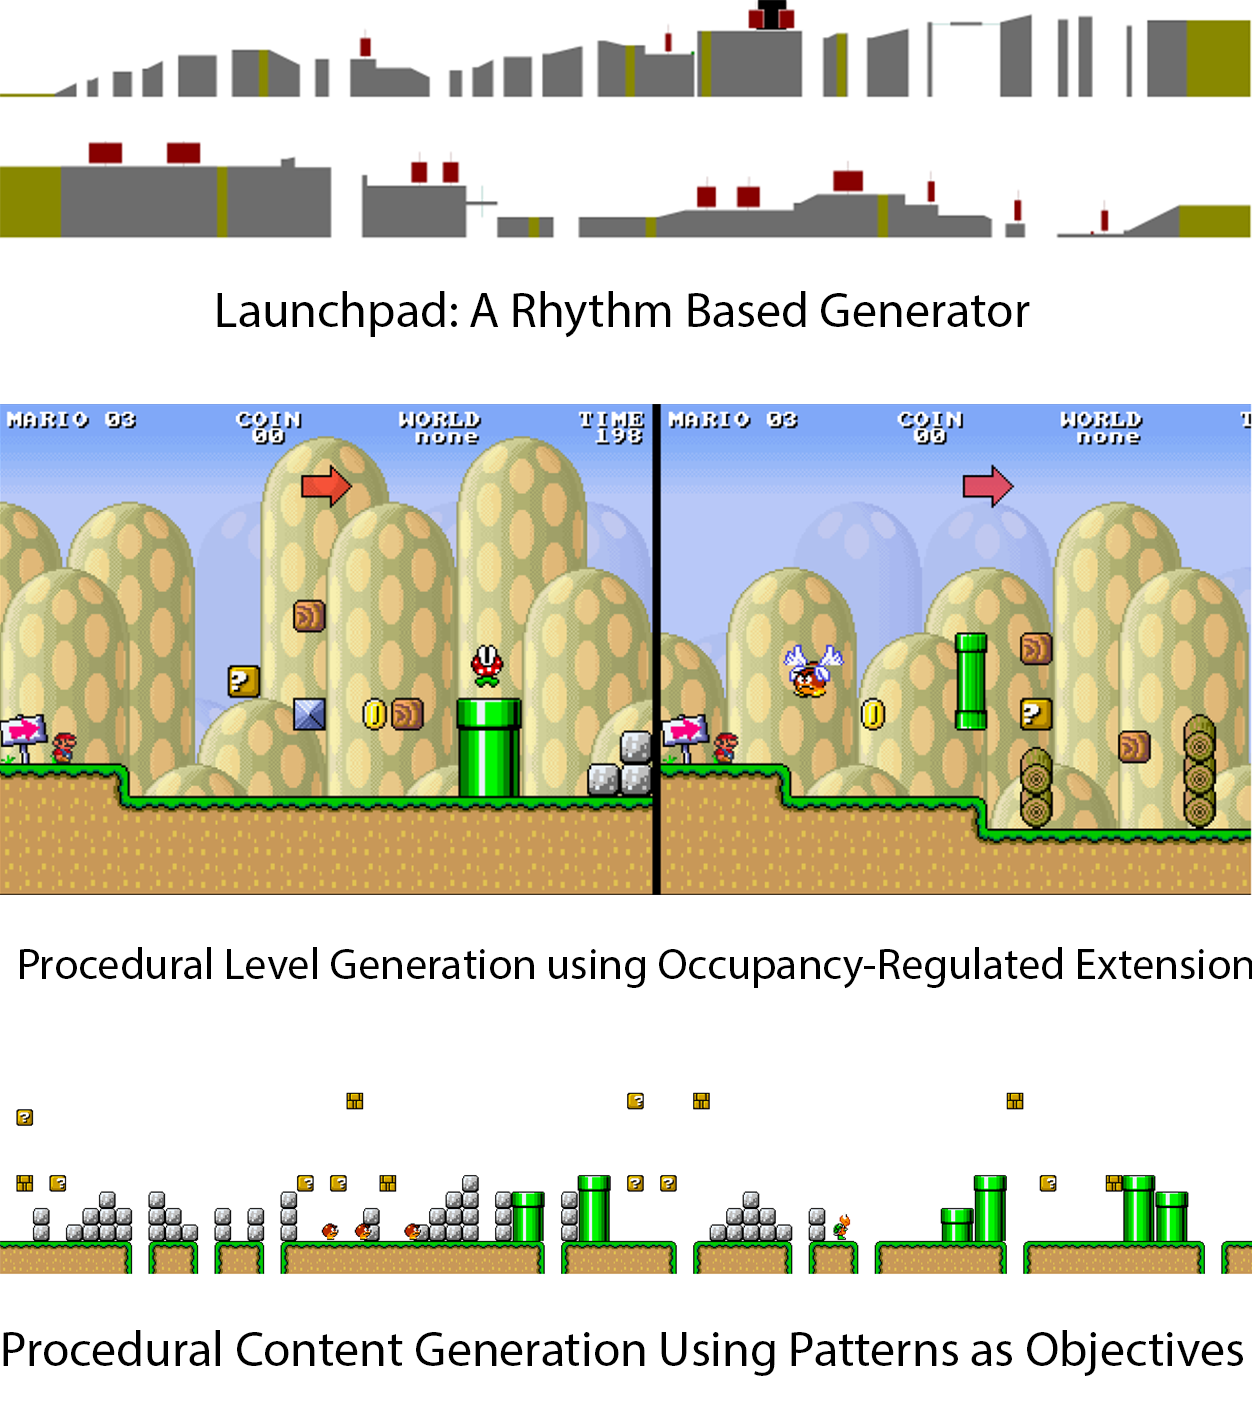
\includegraphics[width=0.75\textwidth]{archtecture-images}
\centering
    \caption{Examples of the PCG levels (figures from \cite{smith2010}, \cite{mawhorter2010} and \cite{dahlskog2014})}
    \label{fig:PCG}
\end{figure}

Figure \ref{fig:PCG} shows a set of images displaying the different outputs of each PCG.

Dahlskog and Togelius provide a good balance between variability and control. However this too has no method of guaranteeing playability when generating a level \cite[p.4]{dahlskog2014}, and also requires a large chunk library in order to work. Furthermore increasing this chunk library will lead to slight performance issues.

Mawhorter and Mateas' ORE produces levels with a lot of variety, which would be appropriate for a exploration style game where getting stuck isn't an issue. However for the context of this paper, that is an undesirable property.

Smith et al. provides the most appropriate solution for this paper, as Launchpad produces levels with very little human authored content and can guarantee playability of each level it generates. It also provides the designer with a large amount of control over the geometry of each level. This method is arguably the most extensible, as the designer has a large ammount of control over the PCG. Also the generator is able to run at runtime as it can generate levels in under a second \cite[p.8]{smith2012web}.



\section{Conclusion}

Overall Launchpad provides a fast PCG that will allow for the indie developers to create levels with minimal effort, while allowing for a large ammount of control over the linearity and leniency of the content that is generated. Also the speed at which it generates levels means it can run within the game engine at runtime.


However for other contexts this recommendation may change.



%Write your conclusion here. The conclusion should do more than summarise the essay, making clear the contribution of the work and highlighting key points, limitations, and outstanding questions. It should not introduce any new content or information.

\bibliographystyle{ieeetr}
\bibliography{comp110_architecture}

\end{document}
